% RoboCupJunior technical description paper starter
% Lines beginning with % are writing and LaTeX tips. They do not appear in the PDF.
% This paper describes a fictional robot and fictional test results.
% Replace all example text, images and results with your own work.
% Use only the sections and examples that fit your project and event.
\documentclass[runningheads]{llncs}
\usepackage[T1]{fontenc}
\usepackage[utf8]{inputenc}
\usepackage{graphicx} % Include images from files.
\usepackage{float}    % Keep an example figure near its explanation.
\usepackage{amsmath}  % Extra tools for equations.
\usepackage{url}      % Format web addresses in references.

% Replace these placeholders. Ask your team which names can be shared.
\title{Pebble: A Small Robot on a Rescue Line}
\titlerunning{Pebble the Rescue Robot}
\author{Team Lost Socks}
\authorrunning{Team Lost Socks}
\institute{The Imaginary Robotics Club \\ {Example Region}}

\begin{document}
\maketitle

\begin{abstract}
% Introduce your project in one short paragraph. What does it do? Describe
% important design choices and what you learned. You can write this last.
Pebble is a fictional RoboCupJunior Rescue Line robot. It follows a dark line
and uses a distance sensor to spot obstacles. We compared two speeds on a
practice course and found that the slower setting helped Pebble stay on track.
Pebble is still learning that a shadow is not a shortcut.

% Keywords help readers find your paper. Separate them with \and.
\keywords{Robotics \and Design \and Testing}
\end{abstract}

\section{Team and goals}
% Introduce your team and project. What did you want to achieve? Describe each
% team member's contribution. Include names only if appropriate for your event.
% A citation gives credit to a source. Replace this sample citation with your
% own, or remove it and its bibliography entry. The key in \cite{...} must
% match the key in \bibitem{...} at the end of this file.
Team Lost Socks is a fictional team of three students. Ada designed the
chassis, Bo worked on the sensors, and Cy programmed the robot's movement.
We built Pebble to follow a line and navigate a practice rescue course.
The project is imaginary, including the test results in this example.
RoboCupJunior brings together several robotics leagues~\cite{rcj}.

\section{System overview}
% Describe the whole system and how its main parts work together.
% The following image is an example. Replace the image file and caption with
% your own diagram or photo. Refer to the figure in the text using \ref.
% Upload your image to the figures folder. PDF, PNG and JPG work with pdfLaTeX.
% Change the file name below to match yours, including capital letters.
Pebble uses sensors to find the line and nearby obstacles, a controller to
decide what to do, and motors to move. Figure~\ref{fig:pebble} shows our imaginary robot.
Figure~\ref{fig:system} shows how information moves through the system.

% This example illustration was generated for this starter. Replace it with
% your own photograph or drawing and describe what readers should notice.
\begin{figure}[H]
  \centering
  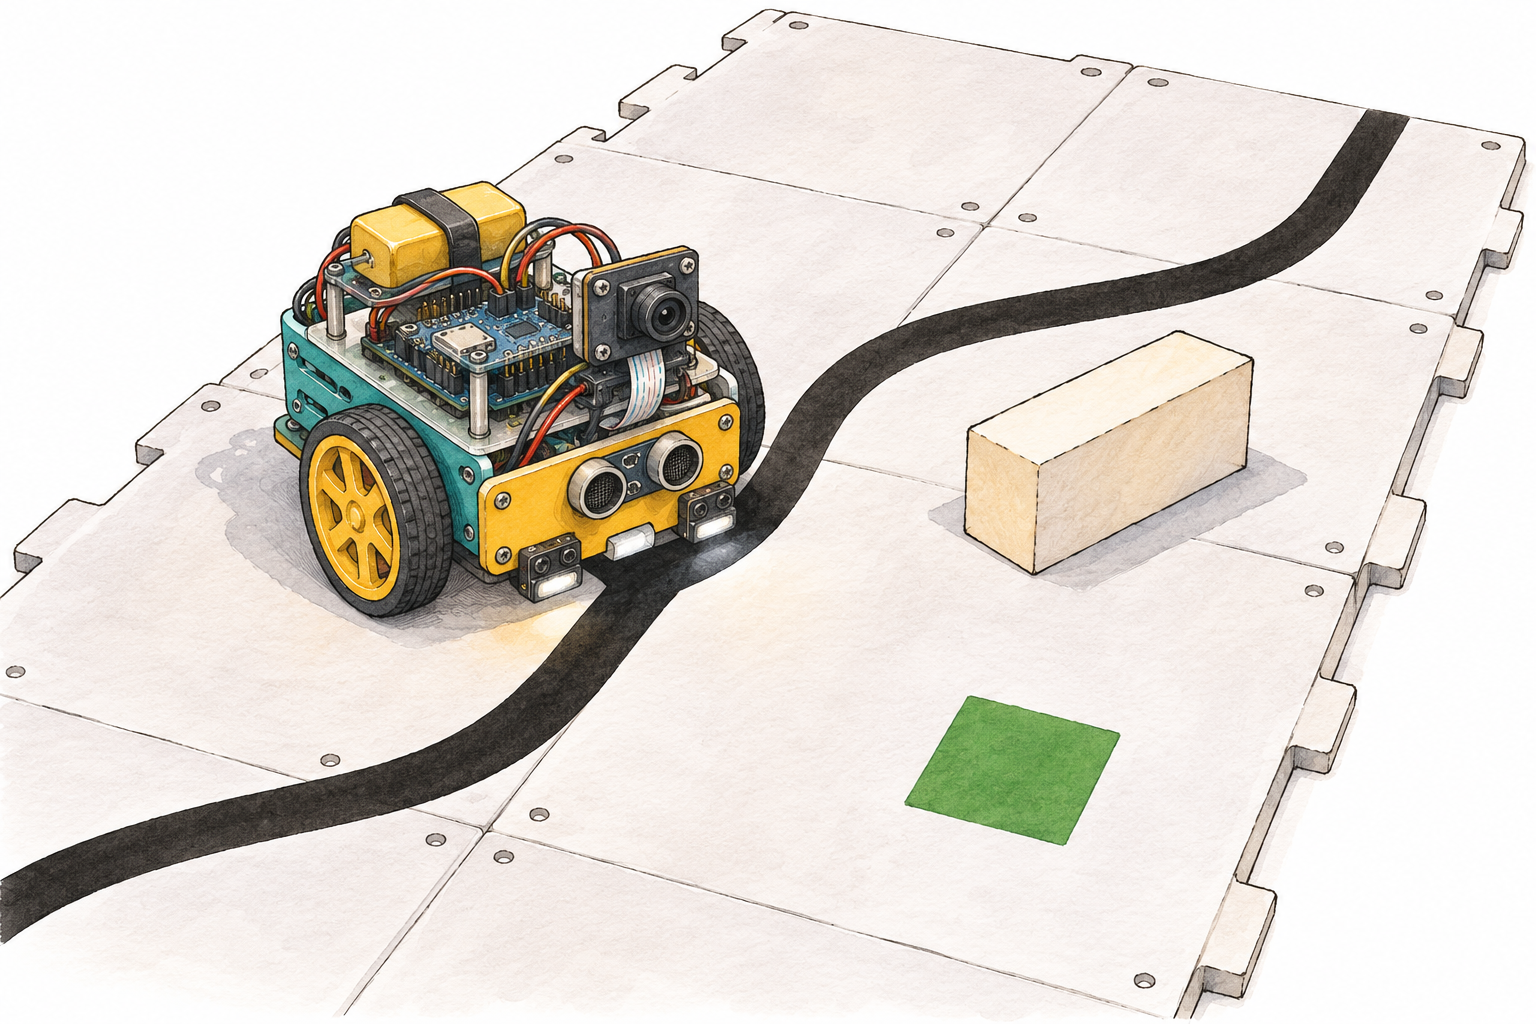
\includegraphics[width=0.68\textwidth]{figures/pebble.png}
  \caption{An imagined Rescue Line practice course and our fictional robot, Pebble.}
  \label{fig:pebble}
\end{figure}
\begin{figure}[H]
  \centering
  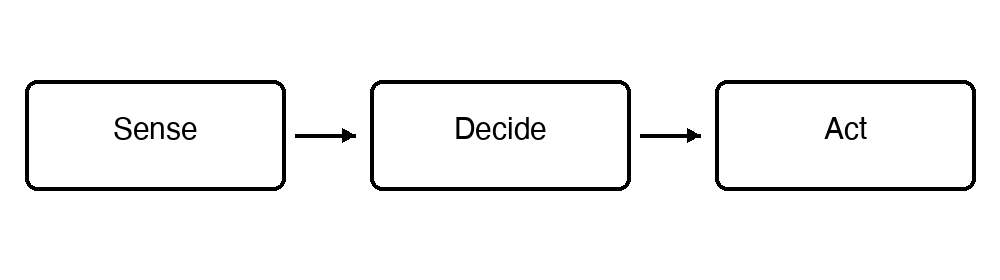
\includegraphics[width=0.85\textwidth]{figures/example-system.png}
  \caption{Pebble reads its sensors, decides what to do and moves.}
  \label{fig:system}
\end{figure}

\section{Design and implementation}
% Explain the parts that matter most: physical structure, electronics, a
% simulated robot, software or performance interactions. What did you build
% or change, and why? Simulation: how is your robot configured and what can
% it sense?
\subsection{Keeping the line in sight}
% Explain how the feature works and what problem it solves. Add subsections
% for other features. OnStage: how does each feature contribute to the show?
We placed line sensors near the front of the chassis. Their readings help
Pebble steer back towards the dark line when it starts to wander. We mounted
the sensors close to the floor to reduce the effect of room lighting.

\section{Behavior and strategy}
% Explain how your system senses, decides and acts. A flowchart can help.
% Choose the following prompts that fit your project:
% Soccer: How do robots find the ball, move on the field and play different roles?
% Rescue Line: How does the robot follow the line, handle gaps and obstacles,
%   and find and handle objects in the evacuation area?
% Rescue Maze: How does the robot navigate, track the maze and respond to victims?
% Rescue Simulation: How does the program navigate, map and detect victims?
% OnStage: What happens in the performance? How do robots contribute and
%   interact with people, other robots or their environment?
Pebble follows the line and checks its distance sensor for obstacles. When it
sees an obstacle, it slows down and tries to steer around it. If it loses the
line, it stops and searches instead of racing confidently in the wrong direction.

\section{Development and testing}
% Describe a test or challenge that changed your design. What did you try,
% how did you test it, what happened, and what changed? Give measurements and
% test conditions when you have them. Consider a match, rescue scenario or
% rehearsal. What did it show about reliability? Which scenarios were hard?
%
% This table is an example. Replace the entries with your own measurements,
% or remove the table. Use & between cells and \\ at the end of each row.
% Put the caption before the table and the label after the caption.
We compared two speeds over ten fictional runs each. At the slower speed,
Pebble stayed on the practice line more often (Table~\ref{tab:results}).
\begin{table}[htbp]
  \caption{Fictional line-following results at two speeds.}
  \label{tab:results}
  \centering
  \begin{tabular}{lll}
    \hline
    Speed & Completed runs & Total runs \\
    \hline
    Fast & 6 & 10 \\
    Slow & 9 & 10 \\
    \hline
  \end{tabular}
\end{table}

% An equation can explain a calculation. This example defines success rate.
% Use it only if it fits your work. \label lets you refer to its number.
We calculated the success rate using Equation~\ref{eq:rate}. For the slow
speed, the fictional result is 9/10, or 90\%.
\begin{equation}
  \text{success rate} = \frac{\text{successful runs}}{\text{total runs}}
  \label{eq:rate}
\end{equation}
% Explain how you tested and what a number means. Do not invent results.

\section{Results and reflection}
% What can your system do now? What are its limits? What did you learn and
% what would you like to improve?
% A list can help when the items are truly separate. Replace or remove it.
These example results suggest that Pebble benefits from a slower speed.
We would test more lighting conditions and course layouts next.
Our two main lessons were:
\begin{itemize}
  \item A slower speed can make line following more reliable.
  \item A robot that stops to look again is easier to debug.
\end{itemize}

\section{Credits and resources}
% Identify work, designs, code, libraries and tools from others that you used.
% Explain what your team created or adapted. Include any other disclosures your
% event requires. Add references below for the sources you mention in the paper.
The Pebble illustration was generated for this template. The robot, team and
test results are fictional examples. Replace these credits with your own.

% Thebibliography is a simple way to add references without a separate file.
% Add a \bibitem{key} for each source, then cite it using \cite{key} in the text.
% Replace this example with your sources. Check links and access dates.
\begin{thebibliography}{9}
\bibitem{rcj}
RoboCupJunior: RoboCupJunior home page. \url{https://junior.robocup.org/},
accessed 13 November 2026.
\end{thebibliography}
\end{document}
